\documentclass[12pt,a4paper]{report}
\usepackage[utf8]{inputenc}
\usepackage[T1]{fontenc}
\usepackage{graphicx}
\usepackage{hyperref}
\usepackage{titlesec}
\usepackage{enumitem}

% Title format settings
\titleformat{\chapter}[display]
  {\normalfont\huge\bfseries}{\chaptertitlename\ \thechapter}{20pt}{\Huge}
\titlespacing*{\chapter}{0pt}{50pt}{40pt}

\begin{document}

% Page de garde
\begin{titlepage}
    \begin{center}
        \includegraphics[width=0.4\textwidth]{logoESI.jpg}\\[1cm]

        {\Large \textbf{École des Sciences de l'Information}}\\[0.5cm]
        {\large Transformation Digitale}\\[2cm]

        \fbox{%
            \parbox{1.1\textwidth}{%
                \centering
                {\Huge \textbf{
                \\[0.1cm]
                    RepuSense\\[0.4cm]
                    Stratégie de Transformation Digitale pour\\
                    l'Analyse de la Réputation des Entreprises
                }}\\[0.5cm]
            }%
        }

        \vspace{2cm}
        \textbf{Réalisé par :}\\[0.5cm]
        Mouad Ennasiry\\
        Kamal Saalaoui\\
        Hicham En-Nami\\[1cm]

        \textbf{Encadré par :} Dr. Amine Sennouni\\[1cm]

        {\large Année académique : 2024 -- 2025}

        \vfill
    \end{center}
\end{titlepage}


\tableofcontents

\chapter{Introduction}

\section{Contexte du projet}
Dans l'ère numérique actuelle, la réputation en ligne est devenue un actif stratégique pour toute organisation. Les commentaires, avis et discussions sur les plateformes digitales façonnent la perception publique et influencent directement les décisions des consommateurs et partenaires.

\section{Objectifs de la digitalisation}
Notre projet vise à transformer le processus traditionnellement manuel de surveillance de la réputation en un système automatisé, intelligent et centralisé. Cette digitalisation permet d'extraire des insights précieux à partir de grandes quantités de données textuelles dispersées sur différentes plateformes.

\chapter{Problématique identifiée}

\section{Défis liés à la gestion de la réputation d'entreprise}
La réputation numérique influence significativement la confiance accordée à une entreprise. Cependant, les informations concernant la perception publique sont dispersées à travers un vaste écosystème digital : réseaux sociaux, forums, avis clients, médias en ligne. Cette fragmentation rend la surveillance exhaustive pratiquement impossible avec des méthodes manuelles.

\section{Limites des approches traditionnelles}
Les méthodes traditionnelles de veille d'e-réputation présentent plusieurs limitations :
\begin{itemize}
    \item Processus chronophage nécessitant une surveillance constante
    \item Couverture limitée à quelques canaux spécifiques
    \item Difficulté à analyser systématiquement de grands volumes de textes
    \item Approche principalement réactive plutôt que proactive
    \item Absence d'analyse qualitative approfondie
\end{itemize}

\section{Opportunités offertes par la digitalisation}
La digitalisation offre des opportunités significatives pour surmonter ces défis :
\begin{itemize}
    \item Automatisation de la collecte et du traitement des données
    \item Application de techniques d'analyse textuelle à grande échelle
    \item Centralisation et structuration des informations
    \item Visualisation claire des tendances et thématiques émergentes
\end{itemize}

\chapter{Présentation de la solution RepuSense}

\section{Objectifs fonctionnels et techniques}
RepuSense a été développé avec les objectifs spécifiques suivants :

\begin{enumerate}
    \item \textbf{Centralisation des données} : Créer un point unique de collecte et d'analyse pour les mentions d'une entreprise.
    \item \textbf{Analyse textuelle} : Appliquer des techniques de NLP pour évaluer le sentiment, identifier les thèmes dominants et extraire des mots-clés pertinents.
    \item \textbf{Visualisation intuitive} : Développer une interface utilisateur permettant de comprendre rapidement les tendances et insights.
    \item \textbf{Organisation structurée} : Mettre en place un système pour stocker et organiser les données d'analyse.
    \item \textbf{Automatisation de base} : Réduire le temps et les ressources nécessaires à la veille d'e-réputation.
\end{enumerate}

\section{Vue d'ensemble de l'architecture}
L'architecture de RepuSense est conçue pour être modulaire et fonctionnelle :

\begin{figure}[h]
    \centering
    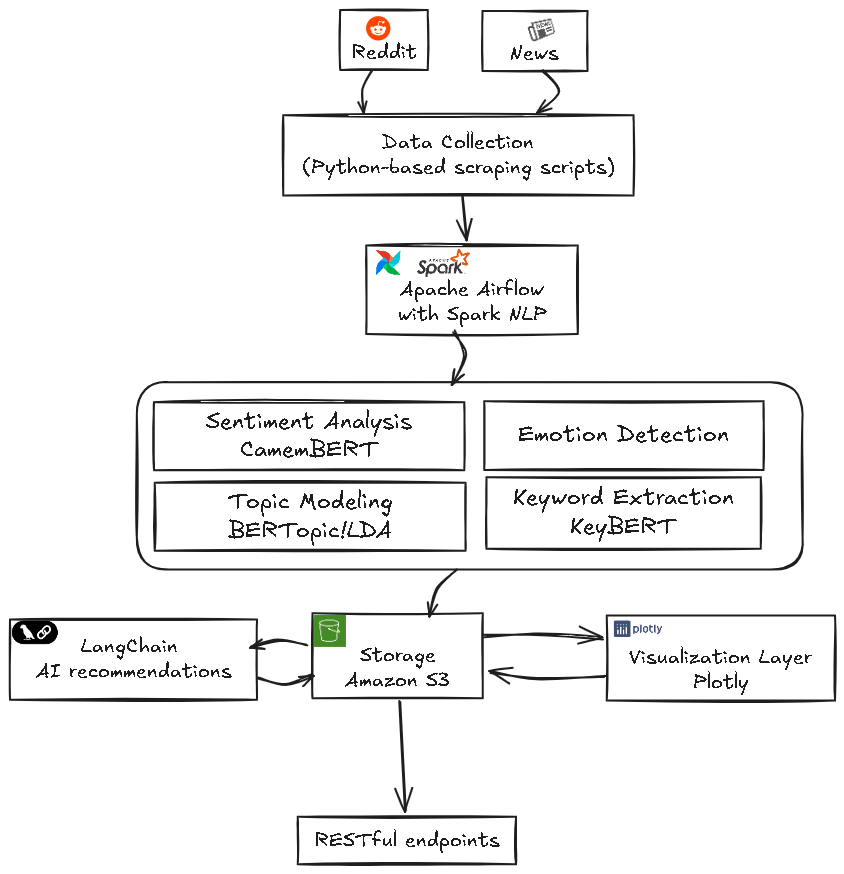
\includegraphics[width=0.8\textwidth]{schema.png}
    \caption{Architecture RepuSense}
\end{figure}

Cette architecture permet de traiter les données depuis leur collecte jusqu'à leur visualisation dans le dashboard, en passant par des étapes d'analyse NLP.

\section{Sources de données exploitées}
RepuSense collecte actuellement des données à partir de :
\begin{itemize}
    \item Reddit (via PRAW - Python Reddit API Wrapper)
    \item Données pré-collectées pour la démonstration
\end{itemize}

Le système est conçu pour être extensible et pourrait intégrer d'autres sources à l'avenir.

\chapter{Axes de digitalisation ciblés}

\section{Automatisation de la veille réputationnelle}
RepuSense digitalise le processus de veille réputationnelle en remplaçant les tâches manuelles par des processus automatisés :
\begin{itemize}
    \item Collecte régulière des données via des scripts programmés
    \item Traitement systématique des nouvelles mentions
    \item Organisation automatique des résultats d'analyse
\end{itemize}

\section{Analyse sémantique via NLP}
L'utilisation des techniques de traitement du langage naturel (NLP) permet d'extraire du sens à partir de grandes quantités de texte :
\begin{itemize}
    \item Analyse de sentiment pour déterminer la tonalité des mentions
    \item Modélisation de sujets pour identifier les thématiques récurrentes
    \item Extraction de mots-clés pour comprendre les termes associés à la marque
\end{itemize}

\section{Visualisation des indicateurs clés}
La transformation des données brutes en visualisations compréhensibles représente un axe clé de la digitalisation :
\begin{itemize}
    \item Tableaux de bord interactifs pour explorer les données
    \item Graphiques et visualisations pour faciliter la compréhension
    \item Organisation visuelle des thématiques et sentiments
\end{itemize}

\chapter{Stratégie de mise en œuvre}

\section{Choix technologiques}
Notre stratégie d'implémentation repose sur l'utilisation de technologies modernes et adaptées :
\begin{itemize}
    \item \textbf{Python} comme langage principal pour le traitement des données et l'analyse NLP
    \item \textbf{Bibliothèques NLP} spécialisées pour l'analyse de texte
    \item \textbf{Next.js et React} pour le développement du dashboard
    \item \textbf{Tailwind CSS} pour l'interface utilisateur
\end{itemize}

\section{Méthodologie de développement}
Le projet a été développé selon une approche itérative :
\begin{enumerate}
    \item Développement initial du pipeline de collecte de données
    \item Implémentation des algorithmes d'analyse NLP de base
    \item Création d'une structure de stockage organisée
    \item Développement du dashboard de visualisation
    \item Intégration des différents composants
\end{enumerate}

\section{Gestion des données et respect de la confidentialité}
La solution a été conçue en tenant compte des aspects éthiques et de confidentialité :
\begin{itemize}
    \item Collecte uniquement de données publiques
    \item Anonymisation des données sensibles
    \item Stockage sécurisé des informations traitées
    \item Respect des conditions d'utilisation des APIs
\end{itemize}

\chapter{Déploiement technique}

\section{Structure du pipeline}
Le pipeline de traitement RepuSense comprend plusieurs étapes séquentielles :
\begin{enumerate}
    \item \textbf{Collecte} : Acquisition des données via des scripts de scraping
    \item \textbf{Prétraitement} : Nettoyage et normalisation des textes
    \item \textbf{Analyse NLP} : Application des algorithmes d'analyse textuelle
    \item \textbf{Stockage} : Organisation des résultats dans une structure cohérente
    \item \textbf{Visualisation} : Présentation des insights via le dashboard
\end{enumerate}

\section{Organisation du traitement}
Le pipeline est implémenté dans le module \texttt{nlp\_pipeline} et peut être exécuté via \texttt{run\_pipeline.py}, qui offre diverses options de configuration :
\begin{itemize}
    \item Sélection de l'entreprise à analyser
    \item Utilisation de données existantes
    \item Choix des analyses à effectuer (sentiment, sujets, mots-clés)
\end{itemize}

\section{Stockage et intégration des résultats}
Les résultats des analyses sont stockés dans une structure de dossiers organisée :
\begin{itemize}
    \item Structure par entreprise et type d'analyse
    \item Formats standardisés pour les résultats d'analyse
    \item Accessibilité pour le dashboard de visualisation
\end{itemize}

\chapter{Résultats et démonstration}

\section{Exemples d'analyses de sentiment}

\begin{figure}[h]
    \centering
    \includegraphics[width=0.8\textwidth]{placeholder_sentiment_analysis.png}
    \caption{Analyse de Sentiment}
\end{figure}

\section{Thèmes identifiés par topic modeling}

\begin{figure}[h]
    \centering
    \includegraphics[width=0.8\textwidth]{placeholder_topic_modeling.png}
    \caption{Modélisation des Sujets}
\end{figure}

\section{Distribution des sources}

\begin{figure}[h]
    \centering
    \includegraphics[width=0.8\textwidth]{placeholder_source_distribution.png}
    \caption{Distribution des Sources}
\end{figure}

\section{Analyse des tendances}

\begin{figure}[h]
    \centering
    \includegraphics[width=0.8\textwidth]{placeholder_trend_analysis.png}
    \caption{Analyse des Tendances}
\end{figure}

\section{Interface du dashboard}

\begin{figure}[h]
    \centering
    \includegraphics[width=0.8\textwidth]{placeholder_dashboard_overview.png}
    \caption{Dashboard Complet}
\end{figure}

\section{Résumé des problématiques détectées}

\begin{figure}[h]
    \centering
    \includegraphics[width=0.8\textwidth]{placeholder_problem_summary.png}
    \caption{Résumé des Problèmes}
\end{figure}

\chapter{Limites et perspectives}

\section{Contraintes techniques rencontrées}
Le développement de RepuSense a permis d'identifier plusieurs défis techniques :

\textbf{Données Bruitées}
\begin{itemize}
    \item \textbf{Défi} : Les données issues du web contiennent beaucoup de bruit et d'informations non pertinentes.
    \item \textbf{Solution actuelle} : Mise en place d'étapes de nettoyage et de filtrage des données.
\end{itemize}

\textbf{Hétérogénéité des Formats}
\begin{itemize}
    \item \textbf{Défi} : Chaque source présente ses données dans un format différent.
    \item \textbf{Solution actuelle} : Développement d'une structure commune pour normaliser les données.
\end{itemize}

\textbf{Complexité de l'Analyse NLP}
\begin{itemize}
    \item \textbf{Défi} : L'analyse de texte naturel présente de nombreux défis techniques.
    \item \textbf{Solution actuelle} : Utilisation de bibliothèques spécialisées et limitation du champ d'analyse.
\end{itemize}

\textbf{Performance du Traitement}
\begin{itemize}
    \item \textbf{Défi} : Traiter efficacement des volumes importants de texte.
    \item \textbf{Solution actuelle} : Traitement par lots et optimisation des algorithmes les plus coûteux.
\end{itemize}

\section{Améliorations envisagées}
Plusieurs pistes d'amélioration ont été identifiées pour les versions futures :

\begin{enumerate}
    \item \textbf{Intégration de sources supplémentaires} :
    \begin{itemize}
        \item Élargir la collecte à d'autres plateformes sociales
        \item Intégrer des sources d'avis clients et forums spécialisés
    \end{itemize}

    \item \textbf{Enrichissement des analyses} :
    \begin{itemize}
        \item Affiner les modèles de sentiment pour une meilleure précision
        \item Développer des analyses comparatives entre concurrents
    \end{itemize}

    \item \textbf{Évolutions techniques} :
    \begin{itemize}
        \item Optimiser les performances de traitement pour des volumes plus importants
        \item Améliorer l'interface utilisateur avec plus d'interactivité
    \end{itemize}
\end{enumerate}

\section{Scalabilité et adaptation à d'autres secteurs}
La solution RepuSense présente un potentiel d'adaptation à divers secteurs :
\begin{itemize}
    \item Application au domaine de la santé pour l'analyse des retours patients
    \item Adaptation pour le secteur financier et l'analyse des opinions sur les produits bancaires
    \item Utilisation dans le secteur public pour le suivi de l'image des institutions
\end{itemize}

\chapter{Conclusion}

\section{Bilan de la digitalisation apportée}
RepuSense représente une solution pratique au défi de la surveillance de réputation numérique en combinant :
\begin{itemize}
    \item Des techniques d'analyse de texte accessibles
    \item Une architecture structurée et modulaire
    \item Une interface utilisateur intuitive
\end{itemize}

Cette digitalisation permet de transformer un processus manuel, fragmenté et chronophage en un système structuré, centralisé et semi-automatisé.

\section{Apports pour l'entreprise et les parties prenantes}
Cette solution permet aux organisations de :
\begin{itemize}
    \item Mieux comprendre leur présence en ligne
    \item Identifier les tendances importantes dans les discussions
    \item Visualiser les données de réputation de manière claire
    \item Prendre des décisions basées sur des données objectives
\end{itemize}

En transformant des données textuelles en visualisations compréhensibles, RepuSense facilite la gestion de la réputation numérique, un élément désormais essentiel dans l'environnement digital contemporain.

\chapter{Annexes}

\section{Schéma d'architecture du pipeline}
\begin{figure}[h]
    \centering
    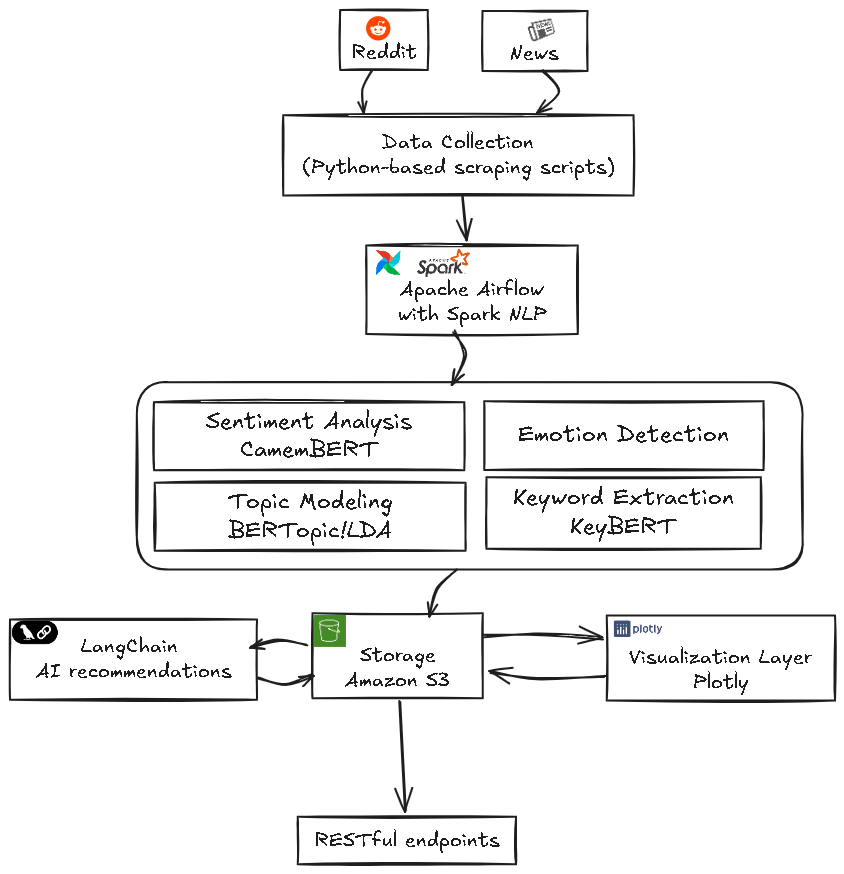
\includegraphics[width=0.8\textwidth]{schema.png}
    \caption{Architecture détaillée}
\end{figure}

\section{Structure du projet}
\begin{verbatim}
RepuSense/
├── config.json                   # Configuration du projet
├── run_pipeline.py               # Script principal
├── nlp_pipeline/                 # Core NLP pipeline code
│   ├── main.py                   # Implémentation du pipeline
│   ├── data_processing/          # Traitement des données
│   └── spark_nlp/                # Composants d'analyse NLP
├── scrapping script/             # Scripts de collecte de données
├── dashboard/                    # Interface utilisateur Next.js
│   ├── app/                      # Pages de l'application
│   ├── components/               # Composants React
│   └── styles/                   # Styles CSS
└── data/                         # Stockage des données
\end{verbatim}

\section{Principales bibliothèques utilisées}
\begin{itemize}
    \item PRAW pour l'accès à l'API Reddit
    \item Bibliothèques NLP pour l'analyse textuelle
    \item Next.js et React pour le frontend
    \item Tailwind CSS pour le design de l'interface
\end{itemize}

\section{Références bibliographiques et techniques}
\begin{itemize}
    \item Documentation de Reddit API
    \item Documentation des bibliothèques NLP utilisées
    \item Ressources sur l'analyse de sentiment et le topic modeling
    \item Documentation de Next.js et React
\end{itemize}

\vspace{1cm}

\end{document} 